A continuacion se presentan las graficas de la superposicion de dos ondas con una fecuencia relativa de 1.05, junto con la regresion de la superposicion por medio de minimos cuadrados.

\begin{figure}[H]
	\centering
	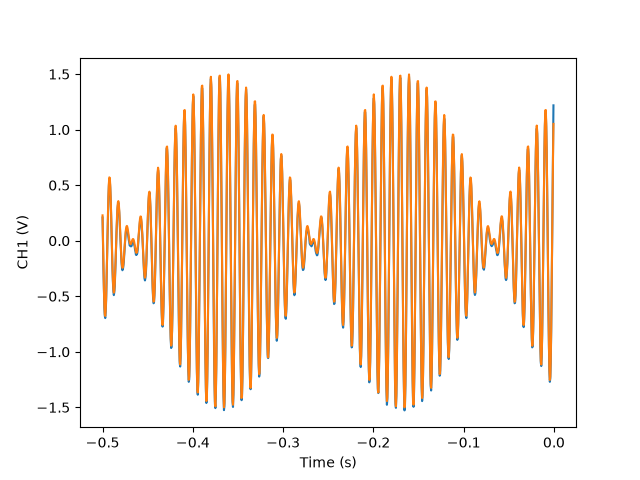
\includegraphics[width=\linewidth]{res/jj1.1.png}
\end{figure}

se presenta ademas los valores reportados por la regresion con sus respectivos errores:
\begin{table}[H]
	\begin{tabular}{c|c|c|c}
		frecuencia & valor teorico (Hz) & valor regresion (Hz) & error (\%) \\ \hline
		$f_0$ & 100 & 100.00128612517261 & 0.00128612517261 \\
		$f_1$ & 105 & 105.00217989423425 & 0.002076089746900661
\end{table}

  

A continuacion se presentan las graficas de la superposicion de dos ondas con una fecuencia relativa de 13, junto con la regresion de la superposicion por medio de minimos cuadrados.

\begin{figure}[H]
	\centering
	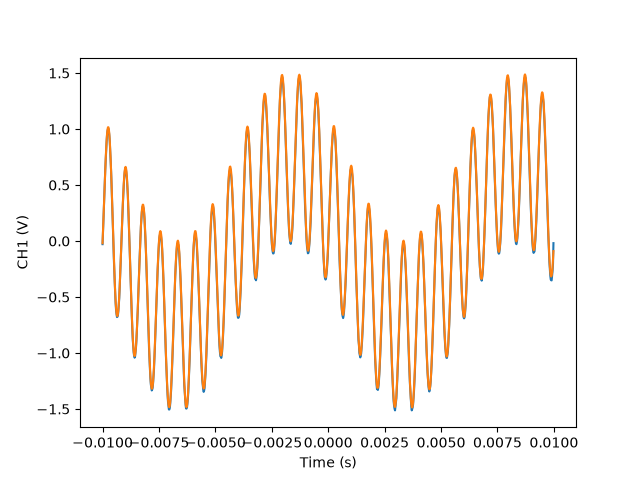
\includegraphics[width=\linewidth]{res/jj13.png}
\end{figure}

se presenta ademas los valores reportados por la regresion con sus respectivos errores:
\begin{table}[H]
	\begin{tabular}{c|c|c|c}
		frecuencia & valor teorico (Hz) & valor regresion (Hz) & error (\%) \\ \hline
		$f_0$ & 100 & 99.77636895729013 & 0.0032601125044318625 \\
		$f_1$ & 1300 & 1300.0423814625576 & -0.2236310427999939
\end{table}


A continuacion se presentan las graficas de la superposicion de cuatro ondas con frecuencias y amplitudes relacionadas por eq.\ref{eq:C} para la onda cuadrada, junto con la regresion de la superposicion por medio de minimos cuadrados.

\begin{figure}[H]
	\centering
	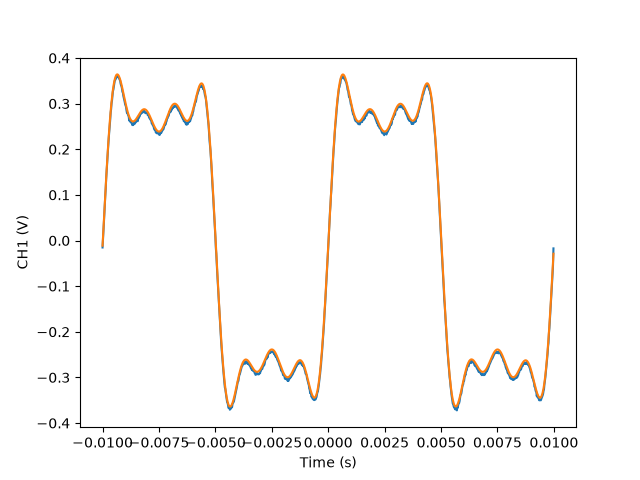
\includegraphics[width=\linewidth]{res/jjc4.png}
\end{figure}

se presenta ademas los valores reportados por la regresion con sus respectivos errores:

\begin{table}[H]
	\begin{tabular}{c|c|c|c}
		valor & valor teorico & valor regresion & error (\%) \\ \hline
		$f_0$ & 100 Hz & 99.9992922 Hz & -0.00071 \\
		$f_1$ & 300 Hz & 300.020043 Hz & 0.00668 \\
		$f_2$ & 500 Hz & 500.078217 Hz & 0.01564 \\
		$f_3$ & 700 Hz & 700.031093 Hz & 0.00444 \\
		$a_0$ & 0.375 V & 0.355697041 V & -5.15 \\
		$a_1$ & 0.125 V & 0.140803539 V & 12.64 \\
		$a_2$ & 0.075 V & 0.0743626350 V & -0.85 \\
		$a_3$ & 0.054 V & 0.0505668770 V & -6.36 \\
\end{table}

A continuacion se presentan las graficas de la superposicion de cuatro ondas con frecuencias y amplitudes relacionadas por eq.\ref{eq:C} para la onda de sierra, junto con la regresion de la superposicion por medio de minimos cuadrados.

\begin{figure}[H]
	\centering
	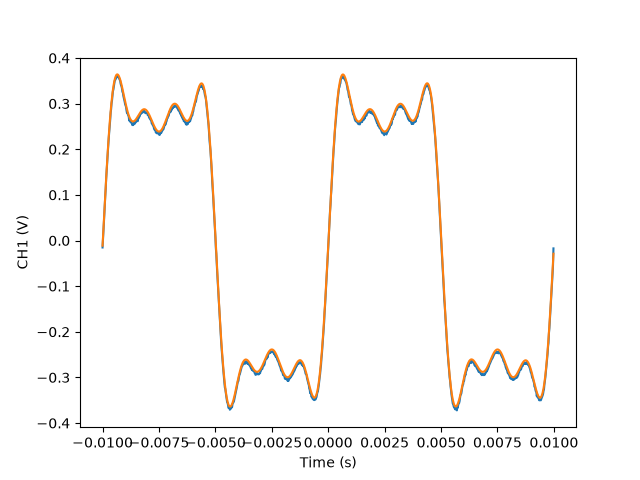
\includegraphics[width=\linewidth]{res/jjc4.png}
\end{figure}

se presenta ademas los valores reportados por la regresion con sus respectivos errores:

\begin{table}[H]
	\begin{tabular}{c|c|c|c}
		valor & valor teorico & valor regresion & error (\%) \\ \hline
		$f_0$ & 100 Hz & 99.9858995 Hz & -0.01410 \\
		$f_1$ & 200 Hz & 200.010186 Hz & 0.00509 \\
		$f_2$ & 300 Hz & 300.026869 Hz & 0.00896 \\
		$f_3$ & 400 Hz & 400.009890 Hz & 0.00247 \\
		$a_0$ & 0.5 V & 0.453917660 V & -9.22 \\
		$a_1$ & 0.25 V & 0.268294681 V & 7.32 \\
		$a_2$ & 0.167 V & 0.158913798 V & -4.84 \\
		$a_3$ & 0.125 V & 0.134810296 V & 7.85 \\
\end{table}
